% Experimental setup (Hiranya, issue #8)
% Needs: booktabs, graphicx. Numbers from results/bert_hparams.json, results/layoutlm_hparams.json and the training logs.

\section{Experimental setup}
\label{sec:setup}

\paragraph{Implementation and hardware.}
Both models are fine-tuned with the Hugging Face Transformers library~\cite{wolf2020transformers} (version 5.22.1) and PyTorch 2.14.1, using its \texttt{Trainer}. We trained on Google Colab on a single NVIDIA Tesla T4 GPU with mixed-precision (fp16) training. The code is in the notebooks \texttt{03\_bert\_text\_only.ipynb} and \texttt{04\_layoutlm.ipynb}, with shared data loading and evaluation code in \texttt{src/}.

\paragraph{Hyperparameters.}
BERT and LayoutLM use exactly the same hyperparameters (Table~\ref{tab:hparams}). They were fixed in advance and not tuned. The LayoutLM notebook reads them from the saved BERT configuration and stops if any value differs, so the two runs cannot drift apart. Both models are base-size Transformers of the same depth and width, start from pre-trained weights, and add a randomly initialised 9-label classifier.

\begin{table}[t]
  \centering
  \small
  \begin{tabular}{ll}
    \toprule
    Hyperparameter & Value (both models) \\
    \midrule
    Pre-trained model   & \texttt{bert-base-uncased} / \texttt{microsoft/layoutlm-base-uncased} \\
    Max.\ sequence length & 512 sub-tokens \\
    Optimiser           & AdamW~\cite{loshchilov2019adamw} \\
    Learning rate       & $5 \times 10^{-5}$, linear decay, no warm-up \\
    Weight decay        & 0 \\
    Batch size          & 8 receipts \\
    Epochs              & 10 (790 optimisation steps) \\
    Precision           & fp16 mixed precision \\
    Random seed         & 42 \\
    \midrule
    Training time (T4)  & BERT 2.3 min, LayoutLM 2.5 min \\
    \bottomrule
  \end{tabular}
  \caption{Training configuration, shared by both models.}
  \label{tab:hparams}
\end{table}

\paragraph{Training protocol.}
SROIE has no official validation split, and with only 626 training receipts we did not set one aside. Instead, both models are trained on the full training split for the fixed number of epochs. There is no early stopping and no checkpoint selection, and the test split is used exactly once, after training. No model weights are kept. Figure~\ref{fig:loss} shows that both models fit the training data smoothly: the training loss falls from about 1 to about 0.003 by the end of training, and LayoutLM's loss is slightly lower than BERT's for most of the run.

\begin{figure}[t]
  \centering
  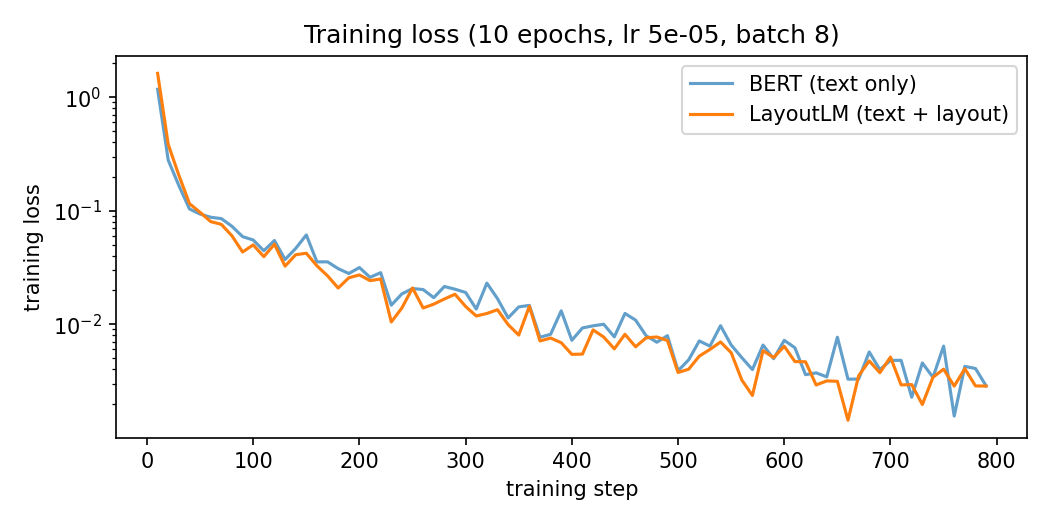
\includegraphics[width=0.7\linewidth]{layoutlm_training_loss.png}
  \caption{Training loss (log scale) of BERT and LayoutLM, logged every 10 steps, with identical hyperparameters.}
  \label{fig:loss}
\end{figure}

\paragraph{Evaluation.}
All three methods (regex, BERT, LayoutLM) are scored with the same field-level evaluation on the 347 test receipts. For each receipt and field, the predicted string is compared with the gold string after normalisation: lowercase, collapse whitespace, strip punctuation at both ends, and for the total also remove a currency prefix (\texttt{RM}) and thousands separators. A prediction is correct only if the two strings are then identical. Per field we report
\begin{equation}
  P = \frac{\#\text{correct}}{\#\text{non-empty predictions}}, \quad
  R = \frac{\#\text{correct}}{\#\text{non-empty gold}}, \quad
  F_1 = \frac{2PR}{P + R},
\end{equation}
and the macro average over the four fields. We use two gold standards (Section~\ref{sec:dataset}). The \emph{main} gold is the string built from the gold word tags, which measures whether a method picks the right words. The \emph{second} gold is the official ICDAR answers; there, even a perfect tagger is capped by OCR noise (Table~\ref{tab:ceiling}). For the two neural models we also report entity-level precision, recall and $F_1$ on the word tags with \texttt{seqeval}~\cite{nakayama2018seqeval}.

\paragraph{Limitations of the setup.}
Each model was trained once with a single seed. Differences of about one $F_1$ point between BERT and LayoutLM on a single field may therefore be within run-to-run variation; repeating the runs with several seeds would make the comparison more robust.
